%\vspace{-0.1in}
\section{Introduction}
\label{sec:intro}

Public cloud providers like Microsoft~\cite{dcqcn} and Google~\cite{timely} are
deploying RoCE in their data centers to enable low latency, high throughput data
transfers with minimal CPU overhead~\cite{dcqcn}. Systems like
Pilaf~\cite{pilaf}, Farm~\cite{farm}, TesnorFlow~\cite{tensorflow}, and
CNTK~\cite{cntk} rely on RoCE for enhanced performance.

RoCE uses Priority Flow Control (PFC) to prevent packet drops due to buffer
overflow at the switches. PFC allows a switch to temporarily pause its upstream
neighbor. While PFC is effective, it can lead to
deadlocks~\cite{rdmaatscale,tcpbolt,hu2016deadlocks}.

Deadlocks in PFC-enabled network are caused by circular buffer dependency
(CBD)~\cite{hu2016deadlocks}. Figure~\ref{fig:deadlock_example}
illustrates a 3-node CBD: switch A is blocked by switch B, which is blocked by
C, which is paused by A. 

The deadlock problem is not merely theoretical -- our conversations with
engineers at large cloud providers confirm that they have seen the problem in
practice and at least one provider has reported it publicly~\cite{rdmaatscale}.
Deadlock is a serious problem because a deadlock is not transient -- once a
deadlock forms, it does not go away even after the conditions (e.g. a temporary
routing loop due to link failure) that caused its formation have
abated~\cite{rdmaatscale}.

Current solutions to the deadlock problem fall in two categories. The first
category consists of solutions that {\em detect} the formation of the deadlock
and then use various techniques to {\em break} it~\cite{shpiner2016unlocking}.
These solutions do not address the root cause of the problem, and hence cannot
guarantee that the deadlock would not immediately reappear. 

The second category of solutions are designed to {\em prevent} deadlocks.  For
deadlock formation, CBD is {\em necessary}, but not {\em
sufficient}~\cite{hu2016deadlocks}. Unfortunately, {\em sufficient} conditions
for deadlock formation are not well understood~\cite{hu2016deadlocks}. Thus,
currently, preventing CBD is the only practical way to prevent deadlocks. 

In \S\ref{sec:challenges}, using data from a large cloud provider's data
centers, we show that any practical deadlock prevention scheme must meet three
key challenges. These include: $(i)$ require no changes to existing routing
protocols or switch hardware, $(ii)$ ability deal with link failures and
associated  route changes, and $(iii)$ availability of limited buffer in
the switches.

While a number of schemes for preventing deadlocks have been proposed, they fail
to meet one or more of these challenges.  Some schemes require centralized,
SDN-style routing.  These are difficult to deploy in existing data centers,
without wholesale infrastructure changes.  Others are distributed, but brand-new
routing protocols~\cite{tcpbolt} that are not supported by commodity switches.
Many of these schemes also require carefully controlling the paths -- something
that is simply not possible with decentralized routing in presence of link
failures~\cite{netpilot}.  Finally, some schemes require creation of numerous
priorities and buffer management according to those priorities. For example, if
each of the flows in Figure~\ref{fig:deadlock_example} had its own priority and
was buffered separately at each switch, there would be no deadlock.  However,
modern data center networks, built using commodity switches, can realistically
support only two or three lossless priorities~\cite{rdmaatscale}.

Thus, to the best of our knowledge, no deadlock free routing solution has been
deployed in a production data center.  In this paper, we present \sysname{},
which meets all three challenges described above, The key insight behind
\sysname{} is that given a topology and a routing protocol, we can enumerate all
paths that need to carry lossless traffic. This task is straightforward for
``structured'' topologies like Clos~\cite{clos}, FatTree~\cite{fattree} and
Bcube~\cite{bcube}, and not onerous even for randomized topologies like
Jellyfish~\cite{jellyfish}.  Given these paths, we create a tagging and buffer
management scheme that guarantees that there will no CBD, and even under
unforeseen link failures or routing errors (even loops!). The tagging scheme can be
implemented using standard match-action rules.

\sysname{} does not require any changes to the routing protocol. It prevents
deadlock under any failure condition. Even for a Jellyfish topology with 2000
switches, \sysname{} requires just three lossless queues per switch.  In fact,
we prove that for Clos topology,  \sysname{} is optimal in terms of number of
lossless queues required.  We also show how to minimize the number of
match-action rules required to implement \sysname{}.

We have implemented and tested \sysname{} on commodity Arista 7050 Switches with
Broadcom chipsets. The implementation requires carefully addressing the problem
of priority transition (\S\ref{sec:implementation}). Our tests show that
\sysname{} has no performance penalty on datapath. 

\begin{figure}
	\centering
	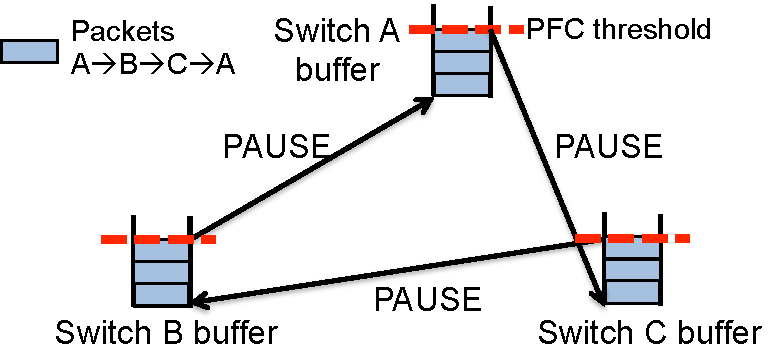
\includegraphics[width=0.5\textwidth] {figs/deadlock}
	\vspace{-0.15in}
	\caption{PFC-induced deadlock: simple illustration of CBD}
	\vspace{-0.15in}
	\label{fig:deadlock_example}
\end{figure}
